\documentclass{article}
\usepackage[utf8]{inputenc}
\usepackage{hyperref}
\usepackage[letterpaper, portrait, margin=1in]{geometry}
\usepackage{enumitem}
\usepackage{amsmath}
\usepackage{booktabs}
\usepackage{graphicx}

\usepackage{hyperref}
\hypersetup{
colorlinks=true,
    linkcolor=black,
    filecolor=black,      
    urlcolor=blue,
    citecolor=black,
}
\usepackage{natbib}

\usepackage{titlesec}

\title{Homework 3}
\author{Roshani Bulkunde}
\date{January 2023}

\begin{document}

\maketitle

\section{Question 1 (a)}

\begin{align}
    y_i &= e^{\alpha}{\delta}^{d_i} z_i^{\gamma} e^{\eta_i}\\
    \text{Take log on both sides } \notag\\
    \ln(y_i) &= \ln(e^{\alpha}{\delta}^{d_i} z_i^{\gamma} e^{\eta_i})\\
    \ln(y_i) &= \ln(e^{\alpha}) + \ln({\delta}^{d_i}) +  \ln(z_i^{\gamma}) +  \ln(e^{\eta_i}) \label{eq:betahat}\\
    \ln(y_i) &= {\alpha}\ln(e) + {d_i} \ln({\delta}) + {\gamma}\ln(z_i) +  {\eta_i}\ln(e) \\
    \text{We know that } \ln(e) = 1 \notag \\
     \ln(y_i) &= {\alpha} + {d_i} \ln({\delta}) + {\gamma}\ln(z_i) +  {\eta_i}
\end{align}

\section{Question 1 (b)}
\subsection{Answer:}
 When both the dependent and independent variables are converted into logs before the OLS estimation, that is the case of elasticity. This is known as the log-log case or double log case and provides us with direct estimates of the elasticities of the independent variables. In this case, the coefficient of estimates is variable.

That means $\delta$ gives the estimates of the elasticities of the variable 'Retrofit'. In other words, coefficient $\delta$ gives the estimates of the difference in the electricity consumption between the houses which received retofit program as compared to the houses which did not receive the program.

\section{Question 1 (c)}
\begin{align}
    y_i &= e^{\alpha}{\delta}^{d_i} z_i^{\gamma} e^{\eta_i}\\
    \text{When } {d_i}=0 \text{   } y_{i0} &= e^{\alpha} z_i^{\gamma} e^{\eta_i}\\
    \text{When } {d_i}=1 \text{   } y_{i1} &= {\delta} e^{\alpha}  z_i^{\gamma} e^{\eta_i}\\
    \bigtriangleup  y_i &= y_{i1} - y_{i0} \\
    \frac{\bigtriangleup  y_i}{\bigtriangleup  d_i} &= ({\delta} _1 - 1) e^{\alpha} z_i^{\gamma} e^{\eta_i}\\
    \text{From equation 6 we can get } e^{\alpha} z_i^{\gamma} e^{\eta_i} &= \frac{y_i}{{\delta}^{d_i}}\\
     \frac{\bigtriangleup  y_i}{\bigtriangleup  d_i} &= \frac{({\delta} _1 - 1)}{{\delta}^{d_i}}  y_i \\
\end{align}

\section{Question 1 (d)}
\begin{align}
    \text{From equation 5 we can get } \notag\\
    \ln(y_i) &= {\alpha} + {d_i} \ln({\delta}) + {\gamma}\ln(z_i) +  {\eta_i} \\
    \text{Differentiate with respect to } z_i \notag \\
    \frac{1}{y_i} \frac{\partial y_i}{\partial z_i} &= \frac{{\gamma}}{z_i}\\
  \frac{\partial y_i}{\partial z_i} &={\gamma} \frac{y_i}{z_i} \\
\end{align}

\section{Question 1 (e)}

\begin{table}[ht]
    \centering
    \begin{tabular}{lrr}
 & Coefficient Estimates & Average Marginal Effect \\
Constant & -0.768728 & 0.000000 \\
Sqft of home & 0.894291 & 0.628662 \\
Retrofit & -0.100547 & -113.975304 \\
Temperature & 0.281345 & 3.997015 \\
Observations & 1000.000000 & 1000.000000 \\
\end{tabular}

    \caption{Estimates table without bootstrapping}
    \label{tab:my_label}
\end{table}

Table \ref{tab:estimates_output} bootstrap the 95\text{\%} confidence intervals of the coefficient estimates and the marginal effects estimates using 1000 sampling replications. Note that each bootstrap replication perform both the regression and the second stage calculation of the marginal effect.
\begin{table}[ht]
    \centering
    \begin{tabular}{lll}
 & Estimates & Average Marginal Effect \\
ln(sqft) & 0.890000 & 0.630000 \\
  & (0.88, 0.91) & (0.62, 0.64) \\
Retrofit & -0.100000 & -113.980000 \\
  & (-0.11, -0.09) & (-129.16, -98.97) \\
ln(Temperature) & 0.280000 & 4.000000 \\
  & (0.05, 0.53) & (0.72, 7.53) \\
Constant & -0.770000 & 0.000000 \\
  & (-1.87, 0.27) & (0.0, 0.0) \\
Observations & 1000 & 1000 \\
\end{tabular}

    \caption{With Bootstrapping}
    \label{tab:estimates_output}
\end{table}

\section{Question 1 (f)}
\begin{figure}[ht]
    \centering
    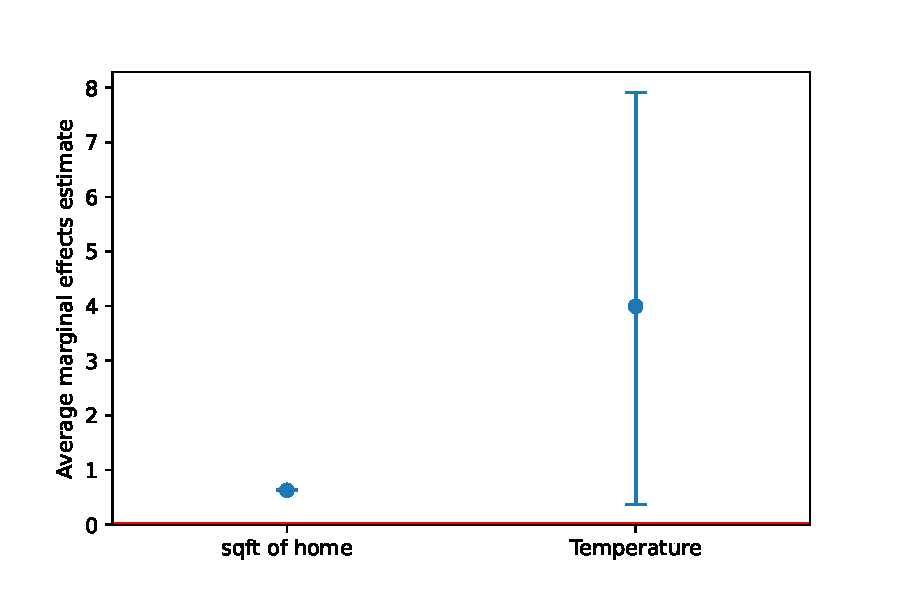
\includegraphics[scale = 0.7]{amebootstrappedCI.pdf}
    \caption{The average marginal effects of outdoor temperature and square feet of the home with
bands for their bootstrapped confidence intervals}
    \label{fig:amebootstrappedCI}
\end{figure}
\end{document}
